\chapter{Πειράματα}\label{ch:experiments}

\section{Τεχνικές προδιαγραφές και εργαλεία}\label{sec:exp-setup}
\subsection{Απαιτήσεις συστήματος}\label{ssec:exp-hardware}
Όλα τα πειράματα της παρούσας εργασίας διενεργήθηκαν σε λειτουργικό σύστημα Ubuntu 22.04.5 LTS, με δύο επεξεργαστές Intel Xeon Silver 4210R (10 πυρήνων στα 2,4\,GHz έκαστος), μία κάρτα γραφικών NVIDIA RTX A6000 με 48\,GB μνήμης GDDR6, και 64\,GB (4$\times$16\,GB) μνήμης RAM DDR4. Τα πειράματα εκτελέστηκαν σε περιβάλλον προσομοίωσης ομοσπονδιακής μάθησης και όχι σε πραγματικές edge συσκευές και ως εκ τούτου, κατέστη απαραίτητη η χρήση ενός μηχανήματος μεγάλης υπολογιστικής ισχύος, ικανού να προσομοιώσει ταυτόχρονα χιλιάδες χρήστες. Σε ένα πραγματικό περιβάλλον, η τοπική εκπαίδευση κάθε client θα μπορούσε να εκτελεστεί βιώσιμα σε edge συσκευές, καθώς το υπολογιστικό της κόστος βρίσκεται εντός των ορίων των περισσότερων σύγχρονων συσκευών.

\subsection{Βιβλιοθήκες και εργαλεία}\label{sec:exp-tools}
Ο κώδικας της εργασίας γράφτηκε σε γλώσσα Python και στηρίχθηκε κυρίως στις βιβλιοθήκες Flower \cite{beutel_flower_2020, flower_software}, PyTorch \cite{paszke_pytorch_2019, pytorch_software} και PyTorch Geometric \cite{fey_fast_2019, pyg_software}.

Το Flower αποτελεί ένα από τα πλέον διαδεδομένα και ολοκληρωμένα open-source frameworks για την ενορχήστρωση ομοσπονδιακής μάθησης, τόσο σε ερευνητικό όσο και σε εμπορικό επίπεδο. Χρησιμοποιείται ως βάση για όλα τα στάδια της προσομοίωσης: από την αρχικοποίηση του server και των clients και τη δέσμευση μνήμης για τη μεταφορά πληροφορίας μεταξύ τους, μέχρι τις συναρτήσεις για aggregation, τους optimizers και τον διαμοιρασμό του συνόλου δεδομένων στους clients. Χωρίς αυτό, η ενορχήστρωση του ομοσπονδιακού περιβάλλοντος θα έπρεπε να υλοποιηθεί χειροκίνητα, εγχείρημα δύσκολο, χρονοβόρο και δευτερεύουσας σημασίας για τους σκοπούς της εργασίας.

Σε παρόμοιο πνεύμα αξιοποιούνται οι βιβλιοθήκες PyTorch και PyTorch Geometric (PyG). Η πρώτη είναι μία από τις θεμελιώδεις βιβλιοθήκες για προβλήματα μηχανικής μάθησης, καθώς παρέχει κλάσεις, βοηθητικές συναρτήσεις και δομές δεδομένων για τη δημιουργία και εκτέλεση μοντέλων, τόσο σειριακά σε επεξεργαστή όσο και παράλληλα σε GPU. Η δεύτερη αποτελεί επέκταση της πρώτης, εξειδικευμένη στη δημιουργία μοντέλων GNN για βαθιά μάθηση σε γράφους.

Συμπληρωματικά χρησιμοποιήθηκαν οι βιβλιοθήκες NumPy \cite{harris_array_2020, numpy_software} και Pandas \cite{mckinney_data_2010, pandas_software} για μαθηματικούς υπολογισμούς και διαχείριση δεδομένων, καθώς και η tqdm \cite{tqdm_software} για την παρακολούθηση της προόδου της εκπαίδευσης, χωρίς ωστόσο να συνεισφέρουν σε κάποια κύρια λειτουργία της υλοποίησης.

\section{Ανάλυση δεδομένων}\label{sec:exp-data}
Όπως περιγράφηκε στην \autoref{ssec:v1-preprocessing}, το σύνολο δεδομένων της Wyze διατίθεται σε δύο ζεύγη αρχείων CSV: ένα για την εκπαίδευση (train) και ένα για την αξιολόγηση (test). Κάθε ζεύγος περιλαμβάνει ένα αρχείο συσκευών και ένα αρχείο κανόνων. Στην παρούσα Ενότητα παρουσιάζεται μια αναλυτική περιγραφή των δεδομένων, από την αρχική μορφή τους έως τις τελικές κατανομές μετά την επεξεργασία και το φιλτράρισμα. Όλα τα μεγέθη που ακολουθούν είναι πλήρως reproducible μέσω του κώδικα της εργασίας \cite{politis_code_2026}.

\subsection{Αρχικά δεδομένα}\label{ssec:data-raw}
Στην ακατέργαστη μορφή τους, τα δύο σύνολα έχουν το μέγεθος που παρουσιάζεται στον Πίνακα \ref{tab:raw-data}. Αξίζει να σημειωθεί ότι τα δύο αρχεία κάθε συνόλου αναφέρονται στους ίδιους ακριβώς χρήστες: το πλήθος των μοναδικών χρηστών στο αρχείο συσκευών ταυτίζεται με εκείνο στο αρχείο κανόνων.

\begin{table}[htbp]
  \centering
  \begin{tabular}{l r r r}
    \toprule
    Σύνολο δεδομένων & Πλήθος χρηστών & Πλήθος συσκευών & Πλήθος κανόνων \\
    \midrule
    Train set & 272.664 & 1.354.098 & 852.072 \\
    Test set  & 13.557  & 110.207   & 60.745  \\
    \bottomrule
  \end{tabular}
  \caption[Μέγεθος ακατέργαστων δεδομένων]{Μέγεθος των συνόλων εκπαίδευσης και αξιολόγησης στην αρχική μορφή της Wyze.}
  \label{tab:raw-data}
\end{table}

\subsection{Λεξιλόγιο}\label{ssec:data-vocab}
Από το σύνολο εκπαίδευσης εξάγεται το λεξιλόγιο όλων των μοναδικών τύπων συσκευών και κανόνων. Τα διαφορετικά μοντέλα συσκευών ανέρχονται σε 16 (15 πραγματικές συσκευές συν το Cloud, που αφορά οποιαδήποτε διασύνδεση με τους servers της Wyze). Ο αριθμός αυτός ορίζει τη διάσταση των one-hot features κάθε κόμβου. Οι διαφορετικοί τύποι κανόνων της μορφής «trigger--action» ανέρχονται σε 791 συνολικά, ωστόσο μετά το φιλτράρισμα των σπάνιων κανόνων (βλ. \autoref{ssec:data-filtering}) διατηρούνται 552, οι οποίοι αποτελούν και τις κλάσεις εξόδου του link predictor. Τέλος, οι μοναδικές καταστάσεις πυροδότησης (trigger states) ανέρχονται σε 45 και οι δράσεις (actions) σε 47. Τα δύο αυτά μεγέθη ορίζουν τις διαστάσεις των αντίστοιχων πινάκων embeddings στις εκδόσεις v2 και v3.

\subsection{Φιλτράρισμα και επαναφορά «φαντασμάτων»}\label{ssec:data-filtering}
Κατά την διαδικασία του preprocessing συμβαίνει μια σειρά διαδοχικών σταδίων φιλτραρίσματος, τα οποία απεικονίζονται στο \autoref{fig:dataset-funnel}. Αρχικά, απορρίπτονται οι κανόνες που εμφανίζονται λιγότερες από 20 φορές συνολικά, ώστε το μοντέλο να εκπαιδευτεί σε συχνά εμφανιζόμενα μοτίβα και όχι σε εξαιρέσεις. Το φιλτράρισμα αυτό γίνεται και στην υλοποίηση της δεύτερης θέσης, με τον αριθμό 20 να είναι καθαρά ενδεικτικός. Το βήμα αυτό αφαιρεί μόλις το 0,3\% των κανόνων (από 852.072 σε 849.618 στο train set). Στη συνέχεια διατηρούνται μόνο οι χρήστες που διαθέτουν τουλάχιστον μία συσκευή και έναν έγκυρο κανόνα (272.397 στην εκπαίδευση), ώστε να απορριφθούν χρήστες με κενούς γράφους. Τέλος, για την εκπαίδευση απαιτούνται τουλάχιστον δύο κανόνες ανά χρήστη ώστε η διαδικασία leave-one-out να αφήνει πάντοτε τουλάχιστον μία ακμή ως context αξιολόγησης, καταλήγοντας σε 149.558 χρήστες. Το ίδιο φίλτρο στο test set δίνει 8.970 χρήστες με $\geq 2$ κανόνες, οι οποίοι αποτελούν το σύνολο cold-start evaluation.

Κατά την ανάλυση των δεδομένων παρατηρήθηκε ότι αρκετές συσκευές συμμετέχουν σε κάποιον κανόνα, ενώ απουσιάζουν από τη λίστα συσκευών του αντίστοιχου χρήστη (οι συσκευές «φαντάσματα» που εισήχθησαν στην \autoref{ssec:v1-preprocessing}). Η συνάρτηση \ident{resurrect_ghosts()} τις επαναφέρει. Η επίδρασή της στο train set μετά το φιλτράρισμα συνοψίζεται στον Πίνακα \ref{tab:ghosts}: η επαναφορά προσθέτει 95.402 ακμές (αύξηση 15,1\%) και διασώζει 8.975 χρήστες που διαφορετικά θα κατέληγαν με κενό γράφο. Αξίζει να αναφερθεί ότι το 96\% των επαναφερόμενων ακμών (91.728) αφορά το Cloud (ειδοποιήσεις, χρονοπρογραμματισμοί κ.ά.) που εξ ορισμού δεν εμφανίζεται στο αρχείο συσκευών (βλ. \autoref{ssec:data-vocab}). Συνολικά, το 12,6\% όλων των ακμών του train set εμπλέκει τη συσκευή Cloud. Χωρίς την επαναφορά «φαντασμάτων», περίπου μία στις οκτώ ακμές θα ήταν μη αναπαραστάσιμη.

\begin{table}[htbp]
  \centering
  \begin{tabular}{l r r r}
    \toprule
    Μέγεθος (μετά το φιλτράρισμα) & Χωρίς resurrection & Με resurrection & Διαφορά \\
    \midrule
    Ακμές train set      & 631.377 & 726.779 & +95.402 \\
    Μη κενοί γράφοι      & 140.583 & 149.558 & +8.975 \\
    Χρήστες με $\geq 2$ ακμές & 123.991 & 149.558 & +25.567 \\
    \bottomrule
  \end{tabular}
  \caption[Επίδραση της επαναφοράς «φαντασμάτων»]{Επίδραση της συνάρτησης \ident{resurrect_ghosts()} στο train set.}
  \label{tab:ghosts}
\end{table}

\begin{figure}[htbp]
  \centering
  \makebox[\linewidth][c]{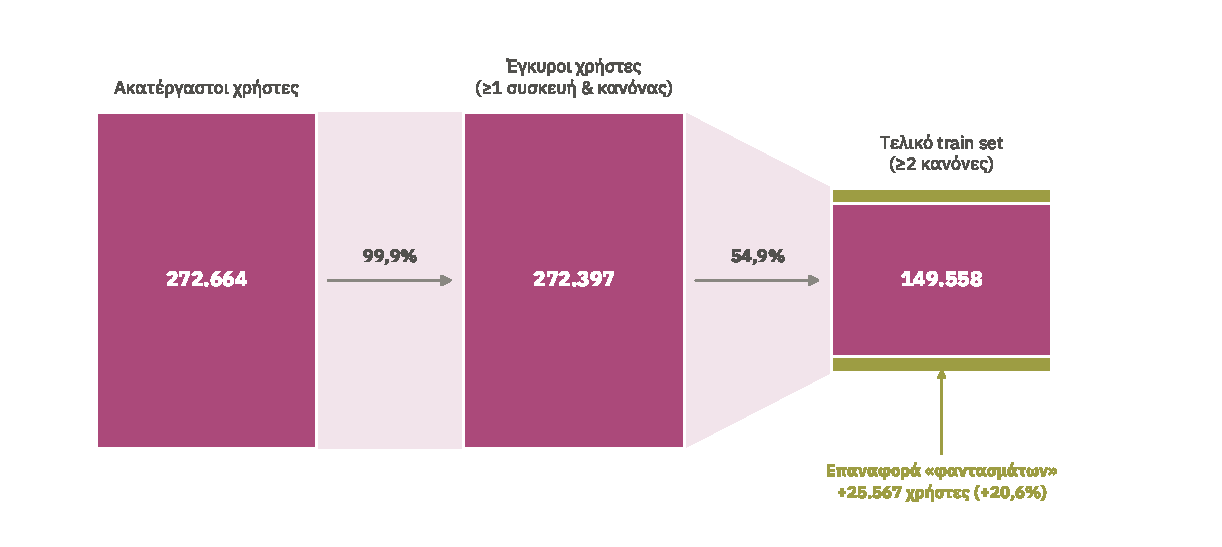
\includegraphics[width=1.2\linewidth]{./assets/images/dataset_funnel}}
  \caption[Διαδικασία φιλτραρίσματος δεδομένων]{Διαδικασία φιλτραρίσματος χρηστών του train set, από τα raw data στα τελικά δεδομένα εκπαίδευσης.}
  \label{fig:dataset-funnel}
\end{figure}

\subsection{Data splits και sampling}\label{ssec:data-splits}
Η εκπαίδευση στην παρούσα εργασία γίνεται στο πλήρες σύνολο των 149.558 χρηστών του train set και η αξιολόγηση γίνεται στο ξεχωριστό αρχείο αξιολόγησης που παρείχε η Wyze (13.544 συνολικοί χρήστες, εκ των οποίων 8.970 με $\geq 2$ κανόνες). Πρόκειται για cold start αξιολόγηση, καθώς οι χρήστες και οι συσκευές του συνόλου αξιολόγησης δεν εμφανίζονται καθόλου στην εκπαίδευση. Αντιθέτως, η υλοποίηση της δεύτερης θέσης χωρίζει το σύνολο εκπαίδευσής της σε αναλογία 80/10/10, εκπαιδεύοντας σε $\sim$119.646 χρήστες και αξιολογώντας σε ένα εσωτερικό, ομοιογενές υποσύνολο $\sim$14.860 χρηστών, μια ουσιώδης διαφορά στο πρωτόκολλο αξιολόγησης που αναλύεται στην \autoref{sec:exp-metrics}.

Για το σενάριο της «καθαρής» cross-device ενορχήστρωσης (περισσότερα στην \autoref{sec:exp-orchestration}), όπου κάθε client αντιστοιχεί σε έναν μόνο χρήστη, το σύνολο εκπαίδευσης υποδειγματοληπτείται σε 25.000 χρήστες χάριν αποδοτικότητας και προσομοίωσης ενός πραγματικού cross-device περιβάλλοντος. Τόσο αυτή η υποδειγματοληψία όσο και κάθε τυχαία επιλογή κατά το preprocessing (π.χ. ο διαμοιρασμός των χρηστών στους clients) βασίζονται σε σταθερό seed, εξασφαλίζοντας ότι κάθε εκτέλεση είναι reproducible και ότι διαφορετικά πειράματα εκπαιδεύονται στο ίδιο ακριβώς υποσύνολο χρηστών.

\subsection{Κατανομές}\label{ssec:data-distributions}
Τα δεδομένα της Wyze χαρακτηρίζονται από έντονη αραιότητα και ετερογένεια, όπως αναλύθηκε θεωρητικά στην \autoref{ssec:fl}. Ο \autoref{tab:distributions} και το \autoref{fig:dataset-stats} ποσοτικοποιούν αυτή την ιδιότητα. Ο διάμεσος χρήστης έχει 3 συσκευές και έχει ορίσει 3 κανόνες, ενώ οι μέσοι όροι (6,19 και 4,86 αντίστοιχα) ανεβαίνουν λόγω μιας μακράς ουράς λίγων «ισχυρών» χρηστών που φτάνουν έως και 154 συσκευές και 446 κανόνες. Το 37,1\% των χρηστών έχει ακριβώς τον ελάχιστο αριθμό των 2 κανόνων, το 77,7\% έχει έως 5, και το 92,5\% έως 10. Εξίσου ασύμμετρη είναι και η κατανομή των ίδιων των τύπων κανόνων: ο πιο δημοφιλής κανόνας εμφανίζεται 65.218 φορές, οι 10 πιο δημοφιλείς τύποι καλύπτουν το 49,8\% όλων των ακμών, ενώ το 50\% των πιο δημοφιλών τύπων καλύπτει το 98,5\% των ακμών.

\begin{table}[htbp]
  \centering
  \begin{tabular}{l r r r r r}
    \toprule
    Μετρική (ανά χρήστη) & Μέσος όρος & Διάμεσος & $\leq 5$ (\%) & $\leq 10$ (\%) & Μέγιστο \\
    \midrule
    Συσκευές & 6,19 & 3 & 70,5 & 83,5 & 154 \\
    Κανόνες  & 4,86 & 3 & 77,7 & 92,5 & 446 \\
    \bottomrule
  \end{tabular}
  \caption[Κατανομές συσκευών και κανόνων ανά χρήστη]{Κατανομές συσκευών και κανόνων ανά χρήστη (train set μετά το φιλτράρισμα). Και οι δύο άξονες παρουσιάζουν έντονη μακρά ουρά (μέσος όρος $\gg$ διάμεσος). Οι στήλες $\leq5$ και $\leq10$ δίνουν το ποσοστό των χρηστών με έως 5 και έως 10 συσκευές ή κανόνες αντίστοιχα.}
  \label{tab:distributions}
\end{table}

\begin{figure}[htbp]
  \centering
  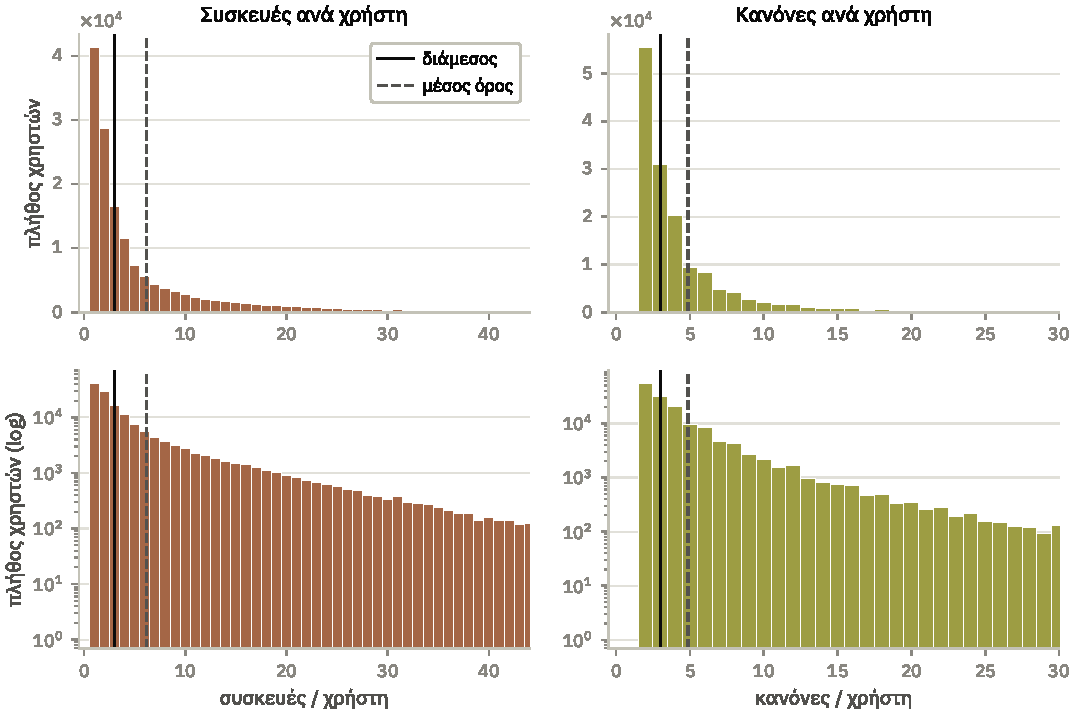
\includegraphics[width=\linewidth]{./assets/images/dataset_stats}
  \caption[Κατανομές συσκευών και κανόνων ανά χρήστη]{Κατανομές του πλήθους συσκευών (αριστερά) και κανόνων (δεξιά) ανά χρήστη, σε γραμμική (επάνω) και λογαριθμική (κάτω) κλίμακα συχνότητας. Ο άξονας $x$ περιορίζεται στο $99^{o}$ εκατοστημόριο για ευκρίνεια. Η μακρά ουρά εκτείνεται πολύ πέρα από αυτό, έως 154 συσκευές και 446 κανόνες ανά χρήστη. Οι κατακόρυφες γραμμές σημειώνουν τη διάμεσο και τον μέσο όρο.}
  \label{fig:dataset-stats}
\end{figure}

\section{Τύποι ενορχήστρωσης}\label{sec:exp-orchestration}
Ένας από τους κυριότερους στόχους της διπλωματικής είναι η κατάδειξη του κόστους που έχει στην αποδοτικότητα πρόβλεψης μία federated υλοποίηση. Για να αξιολογηθεί αυτό πειραματικά, μελετήθηκαν τέσσερα σενάρια ενορχήστρωσης, το καθένα με διαφορετικό βαθμό federation (βλ. \autoref{sec:fl} για τον αρχιτεκτονικό διαχωρισμό μεταξύ cross-device και cross-silo εκπαίδευσης).

\begin{itemize}
    \item \textbf{Centralized:} Αποτελεί το σημείο αναφοράς χωρίς ομοσπονδιακή μάθηση: ένας μοναδικός client κατέχει το σύνολο των δεδομένων όλων των χρηστών και εκπαιδεύει το μοντέλο κεντρικά. Δεν υπάρχει aggregation μεταξύ clients, και επομένως κανένα κόστος που να οφείλεται στην κατανομή των δεδομένων. Χρησιμεύει για να μετρηθεί το «κόστος» της ομοσπονδιακής μάθησης σε επίδοση.
    \item \textbf{Cross-silo:} Τα δεδομένα διαμοιράζονται σε λίγους (4) αξιόπιστους υπερκόμβους (silos), καθένας από τους οποίους κατέχει ένα μεγάλο, ισορροπημένο υποσύνολο χρηστών ($\sim$37.390). Και οι τέσσερις συμμετέχουν σε κάθε γύρο εκπαίδευσης. Το σενάριο αυτό προσφέρει μια ενδιάμεση λύση, μοντελοποιώντας την συλλογή των δεδομένων σε μικρότερους τοπικούς servers σε σχέση με έναν κεντρικό.
    \item \textbf{Pseudo-cross-device με πλήρη δεδομένα:} Μια πρακτικά εφικτή προσέγγιση του cross-device περιβάλλοντος: οι 149.558 χρήστες κατανέμονται σε 2.000 clients ($\sim$75 χρήστες ο καθένας), με πλήρη συμμετοχή ανά γύρο. Το σενάριο διατηρεί την χρήση όλων των δεδομένων, θυσιάζοντας ωστόσο την ιδιότητα «ένας χρήστης ανά client» του πραγματικού cross-device, γι' αυτό και χαρακτηρίζεται «pseudo-cross-device».
    \item \textbf{Πραγματικό cross-device (ένας χρήστης ανά client):} Η πιο πιστή αναπαράσταση του cross-device περιβάλλοντος: το σύνολο υποδειγματοληπτείται σε 25.000 χρήστες, καθένας από τους οποίους αποτελεί ξεχωριστό client (μη-IID γράφος ενός και μόνο χρήστη). Σε κάθε γύρο συμμετέχει μόνο ένα υποσύνολο ($\sim$5.000, δηλαδή 20\%) των clients, όπως συμβαίνει σε πραγματικά δίκτυα εκατομμυρίων συσκευών. Είναι το πιο απαιτητικό σενάριο, καθώς συνδυάζει έντονη ετερογένεια (client drift) με ελάχιστα τοπικά δεδομένα ανά client.
\end{itemize}

\begin{table}[htbp]
  \centering
  \begin{tabular}{l r r r l}
    \toprule
    Σενάριο & Clients & Χρήστες/client & Συμμετοχή/γύρο & Δεδομένα \\
    \midrule
    Centralized                 & 1      & 149.558      & 1 \; (100\%)          & πλήρη \\
    Cross-silo                  & 4      & $\sim$37.390 & 4 \; (100\%)          & πλήρη \\
    Pseudo-cross-device         & 2.000  & $\sim$75     & 2.000 \; (100\%)      & πλήρη \\
    True cross-device           & 25.000 & 1            & $\sim$5.000 \; (20\%) & 25.000 χρ. \\
    \bottomrule
  \end{tabular}
  \caption[Σενάρια ενορχήστρωσης]{Τα τέσσερα σενάρια ενορχήστρωσης. Μόνο το true cross-device σενάριο υποδειγματοληπτεί το dataset.}
  \label{tab:orchestration}
\end{table}

\begin{figure}[htbp]
  \centering
  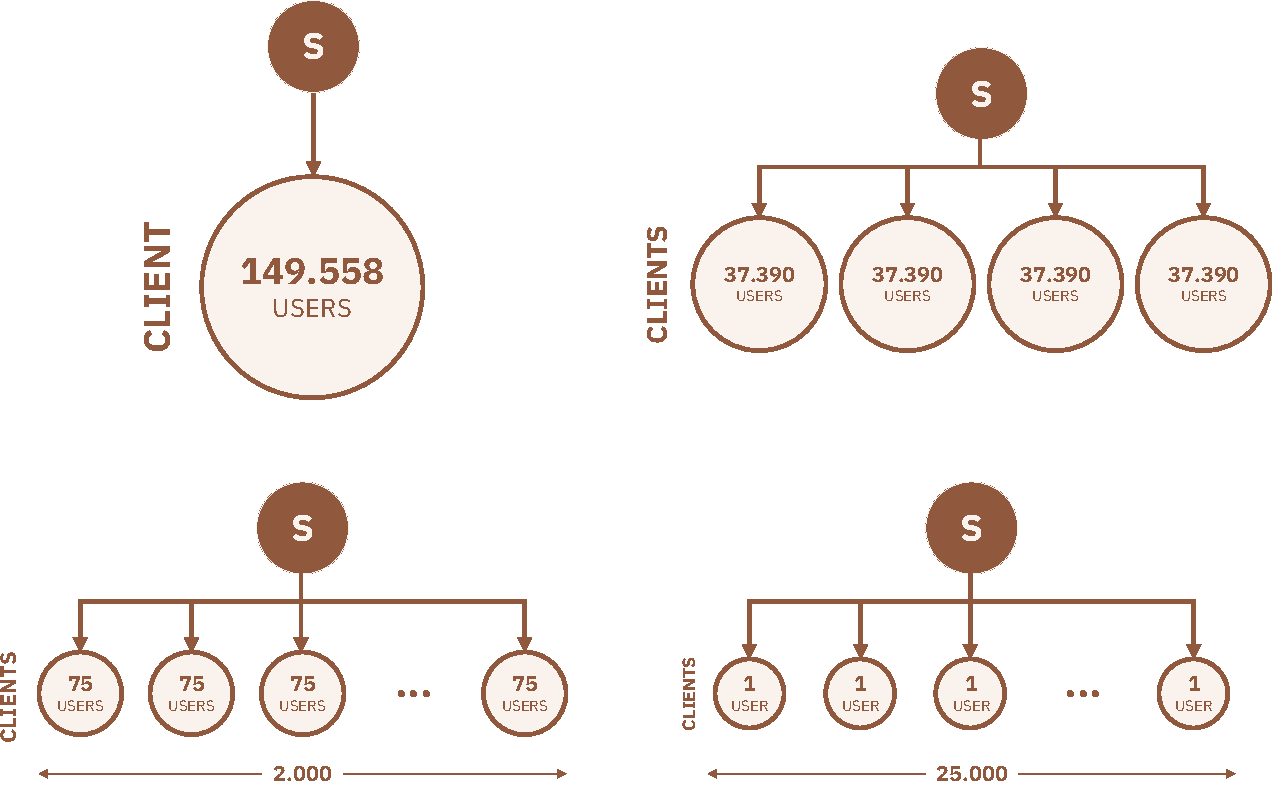
\includegraphics[width=\linewidth]{./assets/images/orchestration}
  \caption[Σενάρια ενορχήστρωσης]{Τα τέσσερα σενάρια ενορχήστρωσης: centralized (πάνω αριστερά), cross-silo (πάνω δεξιά), pseudo-cross-device (κάτω αριστερά) και true cross-device (κάτω δεξιά). Σε κάθε σενάριο, το πλήθος των γράφων χρηστών που ανήκει σε κάθε client μειώνεται ολοένα και περισσότερο, δημιουργώντας ένα ολοένα και πιο federated περιβάλλον.}
\end{figure}

\section{Μετρικές και πρωτόκολλα αξιολόγησης}\label{sec:exp-metrics}
Η αξιολόγηση όλων των μοντέλων γίνεται με ενιαία διαδικασία τύπου leave-one-out, ταυτόσημη με εκείνη που χρησιμοποιείται κατά την εκπαίδευση, ώστε τα δύο στάδια να μην αποκλίνουν. Για κάθε χρήστη του test set αφαιρείται μία ακμή (τριπλέτα «συσκευή-κανόνας-συσκευή»), ενώ οι υπόλοιπες αποτελούν το context που τροφοδοτεί το message passing του GNN. Στην συνέχεια το μοντέλο βαθμολογεί την αφαιρεθείσα ακμή έναντι ολόκληρου του χώρου υποψηφίων του γράφου του χρήστη, όλων δηλαδή των δυνατών permutations των συσκευών που απομένουν επί των 552 τύπων κανόνων, αφού πρώτα αποκλειστούν οι υπόλοιπες γνωστές ακμές. Η θέση (rank) της σωστής τριπλέτας προκύπτει ως το πλήθος των υποψηφίων με αυστηρά υψηλότερη βαθμολογία, συν ένα. Πρόκειται για ένα ιδιαίτερα απαιτητικό πρωτόκολλο, καθώς ο χώρος υποψηφίων ανά χρήστη φτάνει σε τάξη μεγέθους δεκάδων χιλιάδων.

\subsection{Μετρικές}
Ως κύρια μετρική χρησιμοποιείται το Mean Reciprocal Rank (MRR): $$\mathrm{MRR} = \frac{1}{|Q|} \sum_{i=1}^{|Q|} \frac{1}{\mathrm{rank}_i}$$ όπου $Q$ το σύνολο των ακμών που αφαιρέθηκαν και $\mathrm{rank}_i$ το rank της σωστής τριπλέτας για την ακμή $i$. Το MRR κυμαίνεται στο διάστημα $(0,1]$ και ανταμείβει την τοποθέτηση της σωστής πρόβλεψης κοντά στην κορυφή της λίστας.

Συμπληρωματικά αναφέρεται η μετρική HitRate@N: το ποσοστό των ακμών για τις οποίες η σωστή τριπλέτα εμφανίζεται εντός των $N$ πρώτων θέσεων.

\subsection{Πρωτόκολλα αξιολόγησης}
Τα αποτελέσματα εξετάζονται κάτω από δύο πρωτόκολλα, τα οποία αντανακλούν δύο διαφορετικές φιλοσοφίες αξιολόγησης. Η διαφοροποίηση αυτή προκύπτει από το γεγονός ότι η υλοποίηση της δεύτερης θέσης αξιολογεί τον εαυτό της σε ένα λιγότερο αυστηρό, αλλά και λιγότερο ουσιαστικό πλαίσιο.
\begin{itemize}
  \item \textbf{Πλήρες leave-one-out (πρωτόκολλο της εργασίας):} Όλες οι ακμές κάθε χρήστη του test set αφαιρούνται και βαθμολογούνται με τη σειρά, χωρίς όριο στο rank. Πρόκειται για το αυστηρότερο και πιο ειλικρινές μέτρο γενίκευσης γιατί αξιολογεί σε συνθήκες cold-start, με χρήστες και συσκευές που δεν εμφανίστηκαν ποτέ κατά την εκπαίδευση (\autoref{ssec:data-splits}).
  \item \textbf{Πρωτόκολλο δεύτερης θέσης:} Αφαιρείται μία μόνο ακμή ανά χρήστη, επιλεγμένη ντετερμινιστικά μέσω seed, από το 10\% split του train set, και το MRR μηδενίζεται πέραν της 50ής θέσης (MRR@50), υπό την βάση ότι οι συνεισφορές του είναι μηδαμινές.
\end{itemize}
Οι διαφοροποιήσεις αυτές έχουν διπλό αντίκτυπο στο πλαίσιο αξιολόγησης: Αφενός, η αξιολόγηση στο 10\% split του train set αντί για το test set είναι ένα ευκολότερο εγχείρημα, καθώς τα δεδομένα ακολουθούν την ίδια κατανομή με αυτά στα οποία το μοντέλο εκπαιδεύτηκε (in-distribution), και δεν είναι απόλυτα cold-start. Αφετέρου, το γεγονός ότι η αξιολόγηση γίνεται μόνο σε μία, τυχαία επιλεγμένη ακμή κάθε χρήστη και όχι στο σύνολο των ακμών του, την καθιστά μεν σαφώς πιο βιώσιμη υπολογιστικά, αφού δεν εξετάζονται όλα τα πιθανά permutations, αλλά ταυτόχρονα και επιρρεπή στην τυχαιοκρατική φύση της επιλογής ακμής: μπορεί να αφαιρεθεί μία «εύκολη» ακμή από έναν χρήστη, που θα οδηγήσει σε υψηλό rank, ή μία «δύσκολη», που θα υποβαθμίσει το συνολικό αποτέλεσμα. Η εξέταση στο σύνολο των ακμών επιτρέπει την απόλυτα reproducible αξιολόγηση του μοντέλου, ενώ η επιλογή χρηστών από το test set την κάνει ειλικρινή.

Στους πίνακες αποτελεσμάτων, τα δύο πρωτόκολλα συμβολίζονται ως \textbf{full} (πλήρες leave-one-out στο test set, πρωτόκολλο εργασίας) και \textbf{2nd pl.} (πρωτόκολλο δεύτερης θέσης) αντίστοιχα.

\section{Αποτελέσματα}\label{sec:exp-results}
Στην παρούσα Ενότητα συγκεντρώνονται τα αποτελέσματα των τεσσάρων εκδόσεων μοντέλων (2ης θέσης, v1, v2 και v3) υπό τα τέσσερα σενάρια ενορχήστρωσης. Ο \autoref{tab:main-results} συνοψίζει τα αποτελέσματα των πειραμάτων, με κάθε κελί να αναφέρει το MRR υπό τα δύο πρωτόκολλα (full / 2nd pl.).

\begin{table}[htbp]
  \centering
  \begin{tabular}{@{}l cccc@{}}
    \toprule
    Σενάριο & 2η θέση & v1 & v2 & v3 \\
     & (full / 2nd pl.) & (full / 2nd pl.) & (full / 2nd pl.) & (full / 2nd pl.) \\
    \midrule
    Centralized           & 0,2916 / 0,3487 & 0,1505 / 0,1999 & 0,3058 / 0,3574 & \textbf{0,4997 / 0,4956} \\
    Cross-silo            & ---             & 0,1445 / 0,1978 & 0,2950 / 0,3489 & \textbf{0,4598 / 0,4725} \\
    Pseudo-cross-device   & ---             & 0,0649 / 0,0674 & 0,3645 / 0,3287 & \textbf{0,4087 / 0,4127} \\
    True cross-device     & ---             & 0,0733 / 0,0885 & \textbf{0,3791 / 0,4257}$^{\ast}$ & 0,1981 / 0,1716 \\
    \bottomrule
  \end{tabular}
  \caption[Συγκεντρωτικός πίνακας αποτελεσμάτων]{Συγκεντρωτικός πίνακας αποτελεσμάτων: MRR ανά έκδοση μοντέλου και σενάριο ενορχήστρωσης, υπό τα δύο πρωτόκολλα (full~/~2nd pl.). Η στήλη της 2ης θέσης αφορά μόνο κεντρικοποιημένη εκπαίδευση, καθώς η υλοποίησή της δεν έγινε σε federated περιβάλλον. Ο δείκτης $\ast$ σημειώνει ότι η τιμή προέρχεται από μη συγκλίνουσα, ασταθή εκπαίδευση: αποτελεί το βέλτιστο κατά validation μοντέλο και εμφανίζει μεγάλη διακύμανση μεταξύ επαναλήψεων (βλ.\ \autoref{fig:runs-cross-device-true}).}
  \label{tab:main-results}
\end{table}

Οι παρατηρήσεις που προκύπτουν είναι οι εξής:

\begin{itemize}
    \item \textbf{Η αρχιτεκτονική βελτιώνεται:} Η απλούστερη μέθοδος επίλυσης του προβλήματος είναι η v1, καθώς δεν λαμβάνει υπόψιν τους τύπους των ακμών (\autoref{ssec:v1-models}). Ο \autoref{tab:main-results} καταδεικνύει ότι η απόδοση αυτού του μοντέλου είναι η χειρότερη όλων των πειραμάτων (0,1505~/~0,1445~/~0,0649~/~0,0733), και περίπου η μισή του αμέσως επόμενου μοντέλου (0,2916), αυτού της v2 και της 2ης θέσης. Οι υλοποιήσεις αυτές εισάγουν πανομοιότυπα μοντέλα (\autoref{sec:v2}) και φαίνεται πράγματι να καταλήγουν σε παρόμοια απόδοση. Τέλος, οι αρχιτεκτονικές βελτιώσεις της v3 (\autoref{sec:v3}) φαίνεται να έχουν πραγματικό αντίκτυπο στην συνολική απόδοση, με μία αύξηση της τάξης του 71\% στο centralized σενάριο full LOO (0,4997). Επιβεβαιώνεται λοιπόν η θεωρητική διατύπωση ότι ο σχεδιασμός μιας αρχιτεκτονικής εξειδικευμένης στο πρόβλημα που καλείται να επιλύσει συμβάλλει σημαντικά στην αποτελεσματικότητα της εκπαίδευσης.
    \item \textbf{Το κόστος του federation:} Η μελέτη των διαφορετικών σεναρίων ενορχήστρωσης για την v3 αποκαλύπτει ότι υπάρχει ένα υπολογίσιμο αλλά ελεγχόμενο κόστος στην αποδοτικότητα των μοντέλων όσο εισάγεται federation (0,4997 στο centralized σενάριο → 0,4087 στο pseudo-cross-device). Η κατανομή των δεδομένων σε περισσότερους clients με τοπική εκπαίδευση κοστίζει σε επίδοση, ωστόσο εξασφαλίζει όλο και μεγαλύτερη προστασία της ιδιωτικότητας των χρηστών. Εάν συμπεριληφθούν στην μελέτη και οι υπόλοιπες εκδόσεις μοντέλων, το συμπέρασμα για την επιρροή ή μη του federation στην απόδοση δεν είναι ξεκάθαρο.
    \item \textbf{Η αστάθεια του true cross-device σεναρίου:} Όπως είναι φανερό στο \autoref{fig:runs-cross-device-true}, η σύγκλιση του μοντέλου σε ένα εξ ολοκλήρου cross-device περιβάλλον είναι δύσκολη χωρίς την εισαγωγή επιπλέον διορθωτικών παραμέτρων και τον έλεγχο της συνεισφοράς κάθε τοπικού μοντέλου. Η απλούστερη έκδοση v2 φαίνεται να έχει υψηλότερες επιδόσεις από την πιο εξειδικευμένη v3, γεγονός που μπορεί να αποδοθεί εν μέρει στην έλλειψη context εκπαίδευσης που απαιτούν οι μηχανισμοί της v3. Παρουσιάζει ωστόσο και μεγαλύτερη αστάθεια σε σχέση με τις v1 και v3, ωστόσο αυτό πιθανώς οφείλεται στις επιλογές των seed για το συγκεκριμένο πείραμα. Για το cross-device σενάριο διενεργήθηκαν επαναληπτικά πειράματα, τα οποία ωστόσο ήταν εξίσου ασταθή με αυτά που παρουσιάζονται εδώ, και δεν κατέληξαν σε συγκλίνον μοντέλο.
\end{itemize}

\subsection{Καμπύλες σύγκλισης}\label{ssec:exp-convergence}
Οι καμπύλες σύγκλισης ανά γύρο εκπαίδευσης των τριών εκδόσεων σε καθένα από τα τέσσερα σενάρια ενορχήστρωσης, παρουσιάζονται στα Σχήματα \ref{fig:runs-centralized}--\ref{fig:runs-cross-device-true}, ενώ το \autoref{fig:runs-v3-scenarios} συγκρίνει την v3 και στα τέσσερα. Κάθε σχήμα δείχνει τέσσερις καμπύλες ανά γύρο: MRR, HitRate@10, σφάλμα εκπαίδευσης (train loss) και σφάλμα στο σύνολο cold-start (test loss), ενώ η κατακόρυφη διακεκομμένη γραμμή σημειώνει τον γύρο του βέλτιστου μοντέλου που βρέθηκε σε κάθε εκπαίδευση, το οποίο επιλέγεται με κριτήριο τη βέλτιστη MRR στο validation. Οι μετρικές MRR/HitRate@10 αφορούν single-edge αξιολόγηση ανά γύρο στο test set και όχι το τελικό cold-start MRR του Πίνακα \ref{tab:main-results} και χρησιμεύουν για τη μελέτη της σύγκλισης και της σχετικής κατάταξης, όχι των απόλυτων τιμών. Τα αποτελέσματα του Πίνακα \ref{tab:main-results} λήφθηκαν από τα βέλτιστα μοντέλα των διακεκομμένων γραμμών στο validation set.

\begin{figure}[htbp]
  \centering
  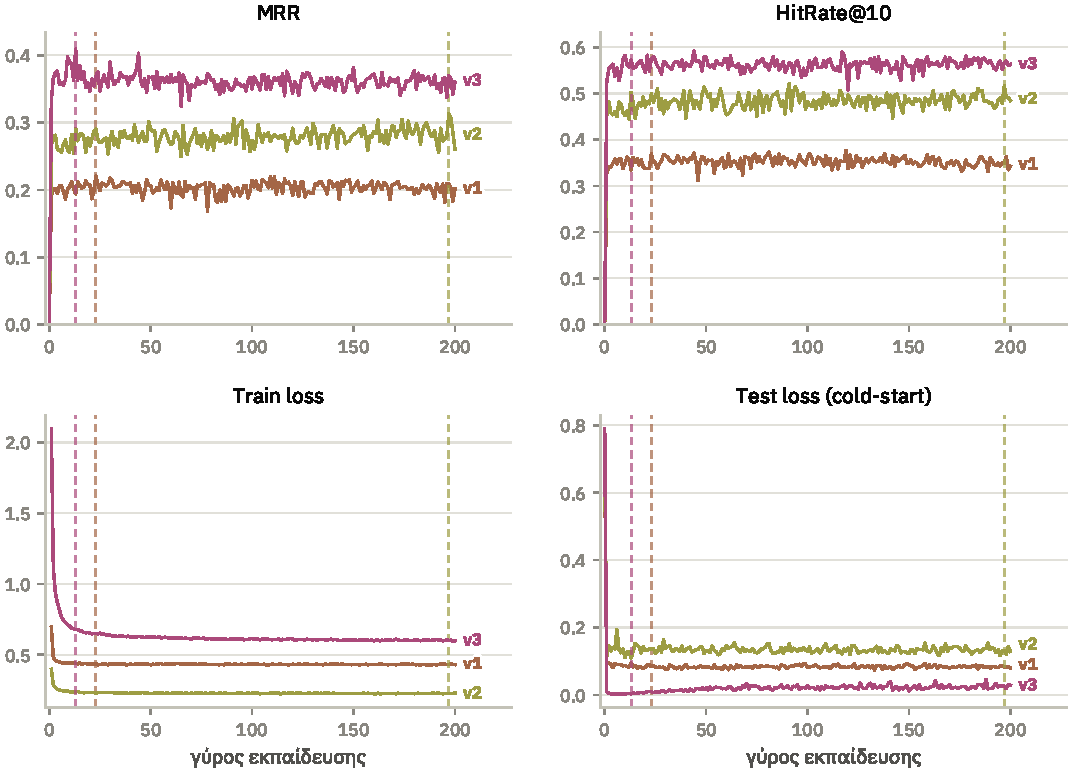
\includegraphics[width=\linewidth]{./assets/images/runs_centralized}
  \caption[Σύγκλιση v1/v2/v3 — centralized]{Σύγκλιση των τριών εκδόσεων στο centralized σενάριο.}
  \label{fig:runs-centralized}
\end{figure}

\begin{figure}[htbp]
  \centering
  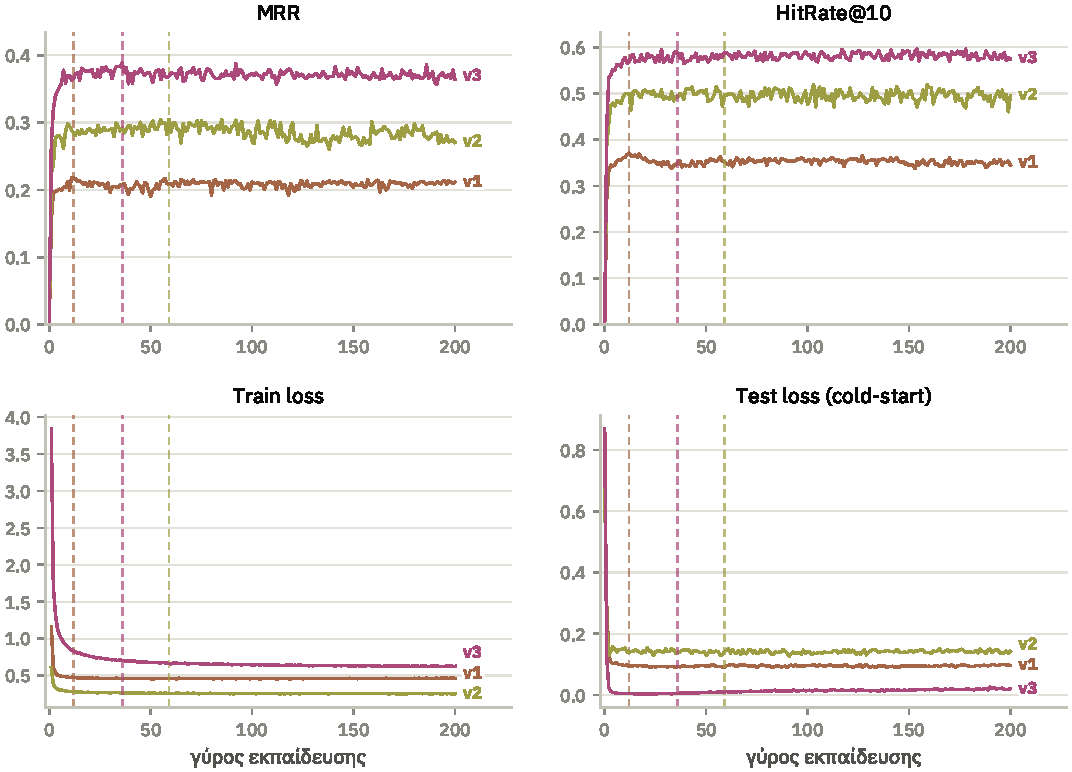
\includegraphics[width=\linewidth]{./assets/images/runs_cross_silo}
  \caption[Σύγκλιση v1/v2/v3 — cross-silo]{Σύγκλιση των τριών εκδόσεων στο cross-silo σενάριο.}
  \label{fig:runs-cross-silo}
\end{figure}

\begin{figure}[htbp]
  \centering
  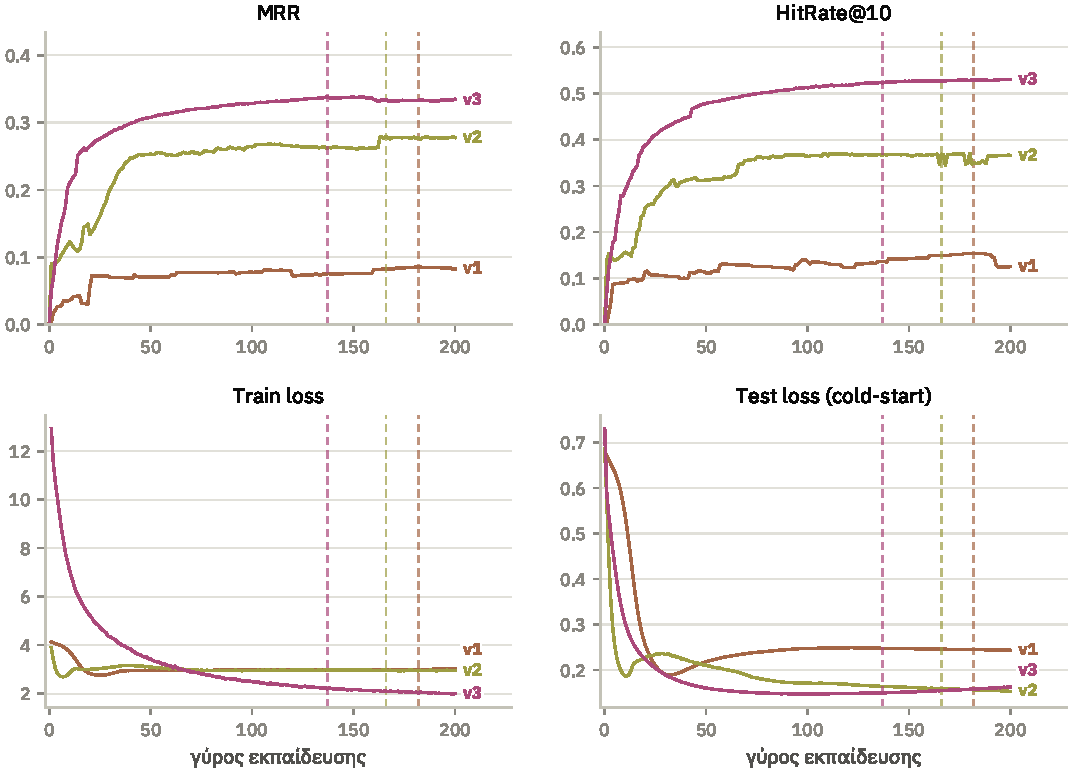
\includegraphics[width=\linewidth]{./assets/images/runs_cross_device_full}
  \caption[Σύγκλιση v1/v2/v3 — pseudo-cross-device]{Σύγκλιση των τριών εκδόσεων στο σενάριο pseudo-cross-device με πλήρη δεδομένα.}
  \label{fig:runs-cross-device-full}
\end{figure}

\begin{figure}[htbp]
  \centering
  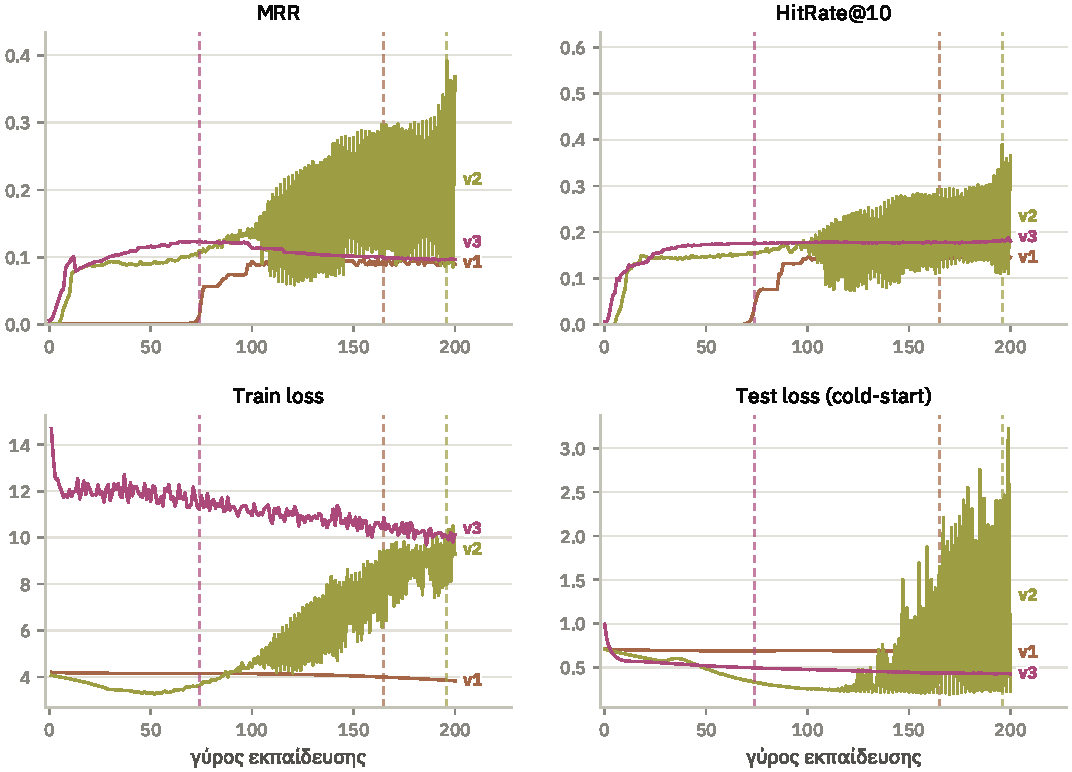
\includegraphics[width=\linewidth]{./assets/images/runs_cross_device_true}
  \caption[Σύγκλιση v1/v2/v3 — true cross-device]{Σύγκλιση των τριών εκδόσεων στο σενάριο true cross-device. Είναι εμφανής η έντονη αστάθεια των καμπυλών, ιδιαίτερα της v2.}
  \label{fig:runs-cross-device-true}
\end{figure}

\begin{figure}[htbp]
  \centering
  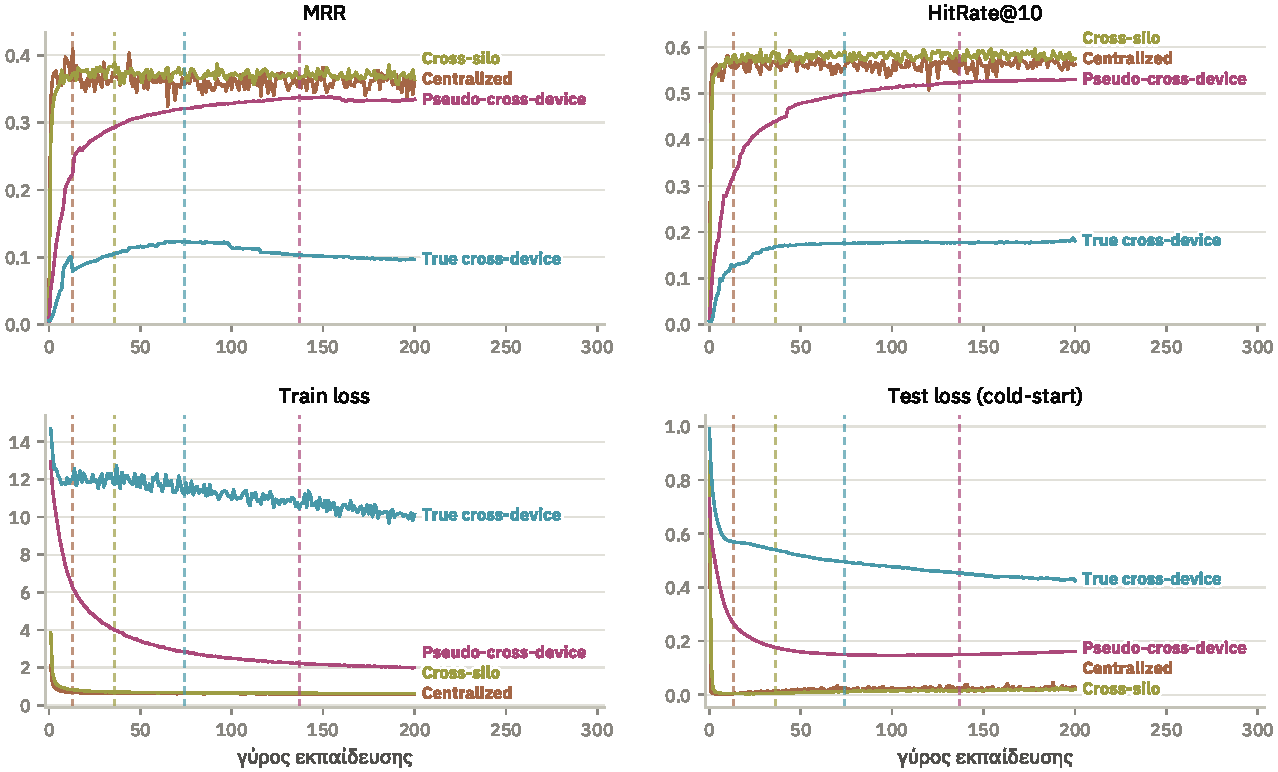
\includegraphics[width=\linewidth]{./assets/images/runs_v3_scenarios}
  \caption[Σύγκλιση της v3 στα τέσσερα σενάρια]{Σύγκλιση της έκδοσης v3 στα τέσσερα σενάρια ενορχήστρωσης: centralized, cross-silo, pseudo-cross-device και true cross-device.}
  \label{fig:runs-v3-scenarios}
\end{figure}

\FloatBarrier
\subsection{Ablation studies}\label{ssec:exp-ablations}
Η τελική σύνθεση της έκδοσης v3 προέκυψε από συστηματικά ablation studies σε μικρότερη κλίμακα (centralized, 10.000 χρήστες, 30 γύροι), οι οποίες απομονώνουν τη συνεισφορά κάθε συνιστώσας. Ο \autoref{tab:ablations} παρουσιάζει τα αποτελέσματα.

\begin{table}[htbp]
  \centering
  \begin{tabular}{l cc}
    \toprule
    Διαμόρφωση & full & 2nd pl. \\
    \midrule
    MLP + BCE (v2)                         & 0,3050 & 0,3066 \\
    MLP + InfoNCE (K=64)                   & 0,2545 & 0,3338 \\
    MLP + BPR (K=64)                       & 0,2466 & 0,3336 \\
    MLP + InfoNCE + hard 50\%              & 0,2732 & 0,3527 \\
    MLP + InfoNCE + hard 100\%             & 0,2029 & 0,2720 \\
    ComplEx + BCE                          & 0,3326 & 0,2807 \\
    DistMult + BCE                         & 0,2969 & 0,2550 \\
    SAGE + ComplEx + InfoNCE + hard 50\%   & 0,3388 & 0,3717 \\
    \textbf{CompGCN + ComplEx + InfoNCE + hard 50\% (v3)} & \textbf{0,4582} & \textbf{0,4369} \\
    \bottomrule
  \end{tabular}
  \caption[Ablation studies]{Ablation studies σε μικρή κλίμακα testing (centralized, 10.000 χρήστες, 30 γύροι). Κάθε γραμμή μεταβάλλει μία συνιστώσα ως προς την τελική σύνθεση.}
  \label{tab:ablations}
\end{table}

Κατά την διαδικασία του ablation, πραγματοποιήθηκαν πειραματισμοί με συνδυασμούς των προαναφερθέντων αρχιτεκτονικών (MLP και SAGE -- \autoref{ssec:v1-models}, BCE -- \autoref{sssec:metrics}, InfoNCE και hard negatives -- \autoref{ssec:infonce}, ComplEx -- \autoref{ssec:complex}), αλλά και με τις επιπλέον προσθήκες των BPR και DistMult.

Η BPR (Bayesian Personalized Ranking) \cite{rendle_bpr_2009} είναι μια συνάρτηση σφάλματος που αξιολογεί ζεύγη ακμών: στόχος της είναι να ταξινομήσει μία θετική ακμή πάνω από μία αρνητική. Υπενθυμίζεται ότι η BCE αξιολογεί μεμονωμένες ακμές (στόχος της δηλαδή είναι να ικανοποιήσει όσο το δυνατόν περισσότερες θετικές ακμές), ενώ η InfoNCE είναι μία συνάρτηση που αξιολογεί λίστα ακμών (στόχος της δηλαδή είναι να ταξινομήσει μία θετική ακμή πάνω από $K$ αρνητικές). Η BPR επομένως αποτελεί μία ενδιάμεση λύση των δύο και αξιολογήθηκε πριν υλοποιηθεί η InfoNCE, ώστε να μελετηθεί αν μία αλλαγή στην συνάρτηση σφάλματος μπορεί να οδηγήσει το μοντέλο σε καλύτερα αποτελέσματα.

Το DistMult \cite{yang_embedding_2015} είναι ένας διγραμμικός embedding decoder με διαγώνιο relation matrix. Αποτελεί relational decoder, όπως το ComplEx, με την διαφορά ότι βαθμολογεί σε πραγματικό διανυσματικό χώρο. Αυτός μάλιστα είναι και ο κυριότερος περιορισμός του, διότι δεν μπορεί να μοντελοποιήσει ασύμμετρες σχέσεις όπως ο μιγαδικός χώρος του ComplEx (\autoref{fig:distmult-complex}). Υπό αυτή την έννοια, το ComplEx αποτελεί γενίκευση του DistMult. Το DistMult λοιπόν αξιολογήθηκε ως ένα πρώτο βήμα στην κατεύθυνση των relational decoders.

Σε γενικές γραμμές, τα ablation studies αναδεικνύουν τα εξής μοτίβα:
\begin{itemize}
    \item \textbf{Alignment πρωτοκόλλου-συνάρτησης σφάλματος:} Οι BPR και InfoNCE είναι συναρτήσεις κατάταξης (έχουν στόχο να τοποθετήσουν την θετική ακμή πάνω από τις αρνητικές), ενώ η BCE όχι (απλώς αξιολογεί θετικές ακμές). Για τον λόγο αυτό, οι πρώτες φαίνεται να βελτιώνουν την απόδοση του μοντέλου στο σενάριο 2nd pl., το οποίο αφαιρεί μόνο μία ακμή και την αξιολογεί (0,338 και 0,336 έναντι 0,3066 της BCE), ενώ η τελευταία κρατά υψηλές τις επιδόσεις στο σενάριο full leave-one-out, όπου αξιολογούνται όλες οι ακμές (0,3050 έναντι 0,2545 και 0,2466 αντίστοιχα). Η επιλογή λοιπόν μίας συνάρτησης σφάλματος εξαρτάται από το σενάριο αξιολόγησης του μοντέλου.
    \item \textbf{Ποσοστό hard negatives:} Η εισαγωγή hard negatives (\autoref{ssec:infonce}) στην εκπαίδευση του μοντέλου φαίνεται να έχει θετικά αποτελέσματα (+2\% έναντι απλού InfoNCE), όμως σε ακραία αναλογία φαίνεται ότι βλάπτουν την εκπαίδευση (-5\% έναντι απλού InfoNCE). Η επιλογή της μερικής εισαγωγής hard negatives θεωρείται βέλτιστη.
    \item \textbf{ComplEx > DistMult:} Η υπόθεση ότι το ComplEx είναι καταλληλότερο για την επίλυση του παρόντος προβλήματος λόγω της δυνατότητάς του να αναπαριστά ασύμμετρες σχέσεις επιβεβαιώνεται. Το ComplEx επικρατεί του DistMult και στα δύο σενάρια (0,3326 vs 0,2969 και 0,2807 vs 0,2550).
    \item \textbf{Η επίδραση του CompGCN:} Η αντικατάσταση του GraphSAGE από το CompGCN επιφέρει την μεγαλύτερη βελτίωση στην επίδοση σε σχέση με όλες τις άλλες τροποποιήσεις μαζί (+12\% στο σενάριο full LOO). Το εύρημα αυτό επιβεβαιώνεται και από το μεμονωμένο ablation του Πίνακα \ref{tab:compgcn-ablation}.
    \item \textbf{Η λύση βρίσκεται στον συνδυασμό μοντέλων:} Καμία λύση δεν δίνει καλύτερες επιδόσεις και στα δύο σενάρια από μόνη της. Η μόνη λύση που πετυχαίνει κάτι τέτοιο είναι ο συνδυασμός μηχανισμών (CompGCN + ComplEx + InfoNCE + hard-50\%). Αυτό σηματοδοτεί ότι οι τροποποιήσεις αυτές δεν δρουν αθροιστικά, αλλά συνεργιστικά.
\end{itemize}

\begin{figure}[htbp]
  \centering
  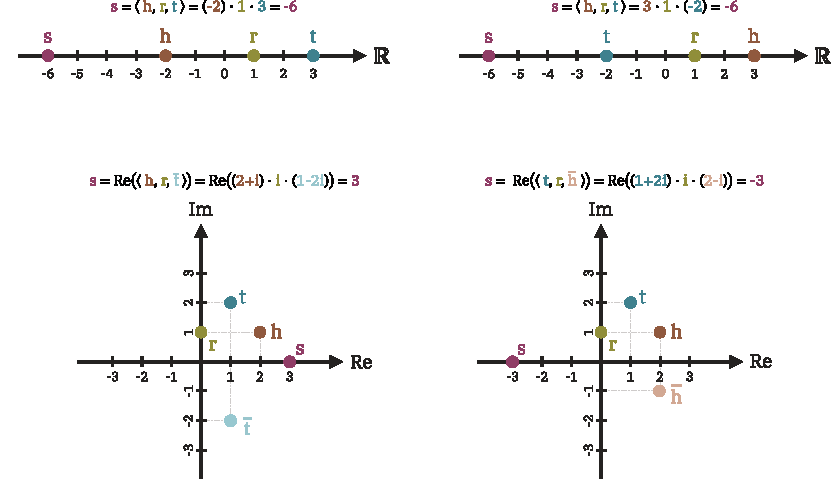
\includegraphics[width=\linewidth]{./assets/images/distmult-vs-complex}
  \caption[DistMult vs.\ ComplEx]{Γιατί ο decoder DistMult δεν μπορεί να αναπαραστήσει κατευθυνόμενες σχέσεις, ενώ ο ComplEx μπορεί. \textbf{DistMult (πάνω, πραγματικός χώρος):} το score $\langle h,r,t\rangle$ είναι ένα απλό γινόμενο τριών πραγματικών αριθμών, οπότε η εναλλαγή των ρόλων $h$ και $t$ αφήνει το αποτέλεσμα αμετάβλητο ($-6$ και στις δύο διατάξεις), λόγω της αντιμεταθετικής ιδιότητας του πολλαπλασιασμού ($a\cdot b=b\cdot a$). Η σχέση είναι αναγκαστικά συμμετρική (δεν μπορεί να διακριθεί ο κανόνας «h→t» από τον «t→h»). \textbf{ComplEx (κάτω, μιγαδικό επίπεδο):} Για τον κανόνα «h→t» (αριστερά) το score $\mathrm{Re}(\langle h,r,\bar t\rangle)=3$ συζυγίζει το tail, ενώ για τον κανόνα «t→h» η συζυγία μεταφέρεται από το $t$ στο $h$ και αλλάζει το score σε $\mathrm{Re}(\langle t,r,\bar h\rangle)=-3$: είναι δηλαδή δυνατή η διάκριση του κανόνα «h→t» από τον «t→h».}
  \label{fig:distmult-complex}
\end{figure}

\textbf{Απομόνωση της συνεισφοράς του CompGCN:} Για να απομονωθεί η συνεισφορά ειδικά του CompGCN, εκτελέστηκε σε πλήρη κλίμακα η έκδοση v3 με αντικατάσταση του GraphSAGE (διατηρώντας ComplEx, InfoNCE και hard negatives). Ο \autoref{tab:compgcn-ablation} δείχνει ότι το CompGCN προσθέτει σημαντική βελτίωση σε όλα τα σενάρια: για παράδειγμα, στο centralized, από 0,3627 (GraphSAGE) σε 0,4997 (CompGCN) υπό το πρωτόκολλο full LOO.

\begin{table}[htbp]
  \centering
  \begin{tabular}{l cc}
    \toprule
    Σενάριο & SAGE + ComplEx + InfoNCE & v3 (CompGCN + ComplEx + InfoNCE) \\
     & (full / 2nd pl.) & (full / 2nd pl.) \\
    \midrule
    Centralized             & 0,3627 / 0,4217 & \textbf{0,4997 / 0,4956} \\
    Cross-silo              & 0,3621 / 0,4293 & \textbf{0,4598 / 0,4725} \\
    Pseudo-cross-device     & 0,3220 / 0,3658 & \textbf{0,4087 / 0,4127} \\
    \bottomrule
  \end{tabular}
  \caption[Συνεισφορά του CompGCN]{Επίδραση της αντικατάστασης του GraphSAGE με CompGCN (σε πλήρη κλίμακα, με σταθερά τα υπόλοιπα στοιχεία της v3).}
  \label{tab:compgcn-ablation}
\end{table}
